\documentclass[1p]{elsarticle_modified}
%\bibliographystyle{elsarticle-num}

%\usepackage[colorlinks]{hyperref}
%\usepackage{abbrmath_seonhwa} %\Abb, \Ascr, \Acal ,\Abf, \Afrak
\usepackage{amsfonts}
\usepackage{amssymb}
\usepackage{amsmath}
\usepackage{amsthm}
\usepackage{scalefnt}
\usepackage{amsbsy}
\usepackage{kotex}
\usepackage{caption}
\usepackage{subfig}
\usepackage{color}
\usepackage{graphicx}
\usepackage{xcolor} %% white, black, red, green, blue, cyan, magenta, yellow
\usepackage{float}
\usepackage{setspace}
\usepackage{hyperref}

\usepackage{tikz}
\usetikzlibrary{arrows}

\usepackage{multirow}
\usepackage{array} % fixed length table
\usepackage{hhline}

%%%%%%%%%%%%%%%%%%%%%
\makeatletter
\renewcommand*\env@matrix[1][\arraystretch]{%
	\edef\arraystretch{#1}%
	\hskip -\arraycolsep
	\let\@ifnextchar\new@ifnextchar
	\array{*\c@MaxMatrixCols c}}
\makeatother %https://tex.stackexchange.com/questions/14071/how-can-i-increase-the-line-spacing-in-a-matrix
%%%%%%%%%%%%%%%

\usepackage[normalem]{ulem}

\newcommand{\msout}[1]{\ifmmode\text{\sout{\ensuremath{#1}}}\else\sout{#1}\fi}
%SOURCE: \msout is \stkout macro in https://tex.stackexchange.com/questions/20609/strikeout-in-math-mode

\newcommand{\cancel}[1]{
	\ifmmode
	{\color{red}\msout{#1}}
	\else
	{\color{red}\sout{#1}}
	\fi
}

\newcommand{\add}[1]{
	{\color{blue}\uwave{#1}}
}

\newcommand{\replace}[2]{
	\ifmmode
	{\color{red}\msout{#1}}{\color{blue}\uwave{#2}}
	\else
	{\color{red}\sout{#1}}{\color{blue}\uwave{#2}}
	\fi
}

\newcommand{\Sol}{\mathcal{S}} %segment
\newcommand{\D}{D} %diagram
\newcommand{\A}{\mathcal{A}} %arc


%%%%%%%%%%%%%%%%%%%%%%%%%%%%%5 test

\def\sl{\operatorname{\textup{SL}}(2,\Cbb)}
\def\psl{\operatorname{\textup{PSL}}(2,\Cbb)}
\def\quan{\mkern 1mu \triangleright \mkern 1mu}

\theoremstyle{definition}
\newtheorem{thm}{Theorem}[section]
\newtheorem{prop}[thm]{Proposition}
\newtheorem{lem}[thm]{Lemma}
\newtheorem{ques}[thm]{Question}
\newtheorem{cor}[thm]{Corollary}
\newtheorem{defn}[thm]{Definition}
\newtheorem{exam}[thm]{Example}
\newtheorem{rmk}[thm]{Remark}
\newtheorem{alg}[thm]{Algorithm}

\newcommand{\I}{\sqrt{-1}}
\begin{document}

%\begin{frontmatter}
%
%\title{Boundary parabolic representations of knots up to 8 crossings}
%
%%% Group authors per affiliation:
%\author{Yunhi Cho} 
%\address{Department of Mathematics, University of Seoul, Seoul, Korea}
%\ead{yhcho@uos.ac.kr}
%
%
%\author{Seonhwa Kim} %\fnref{s_kim}}
%\address{Center for Geometry and Physics, Institute for Basic Science, Pohang, 37673, Korea}
%\ead{ryeona17@ibs.re.kr}
%
%\author{Hyuk Kim}
%\address{Department of Mathematical Sciences, Seoul National University, Seoul 08826, Korea}
%\ead{hyukkim@snu.ac.kr}
%
%\author{Seokbeom Yoon}
%\address{Department of Mathematical Sciences, Seoul National University, Seoul, 08826,  Korea}
%\ead{sbyoon15@snu.ac.kr}
%
%\begin{abstract}
%We find all boundary parabolic representation of knots up to 8 crossings.
%
%\end{abstract}
%\begin{keyword}
%    \MSC[2010] 57M25 
%\end{keyword}
%
%\end{frontmatter}

%\linenumbers
%\tableofcontents
%
\newcommand\colored[1]{\textcolor{white}{\rule[-0.35ex]{0.8em}{1.4ex}}\kern-0.8em\color{red} #1}%
%\newcommand\colored[1]{\textcolor{white}{ #1}\kern-2.17ex	\textcolor{white}{ #1}\kern-1.81ex	\textcolor{white}{ #1}\kern-2.15ex\color{red}#1	}

{\Large $\underline{11a_{193}~(K11a_{193})}$}

\setlength{\tabcolsep}{10pt}
\renewcommand{\arraystretch}{1.6}
\vspace{1cm}\begin{tabular}{m{100pt}>{\centering\arraybackslash}m{274pt}}
\multirow{5}{120pt}{
	\centering
	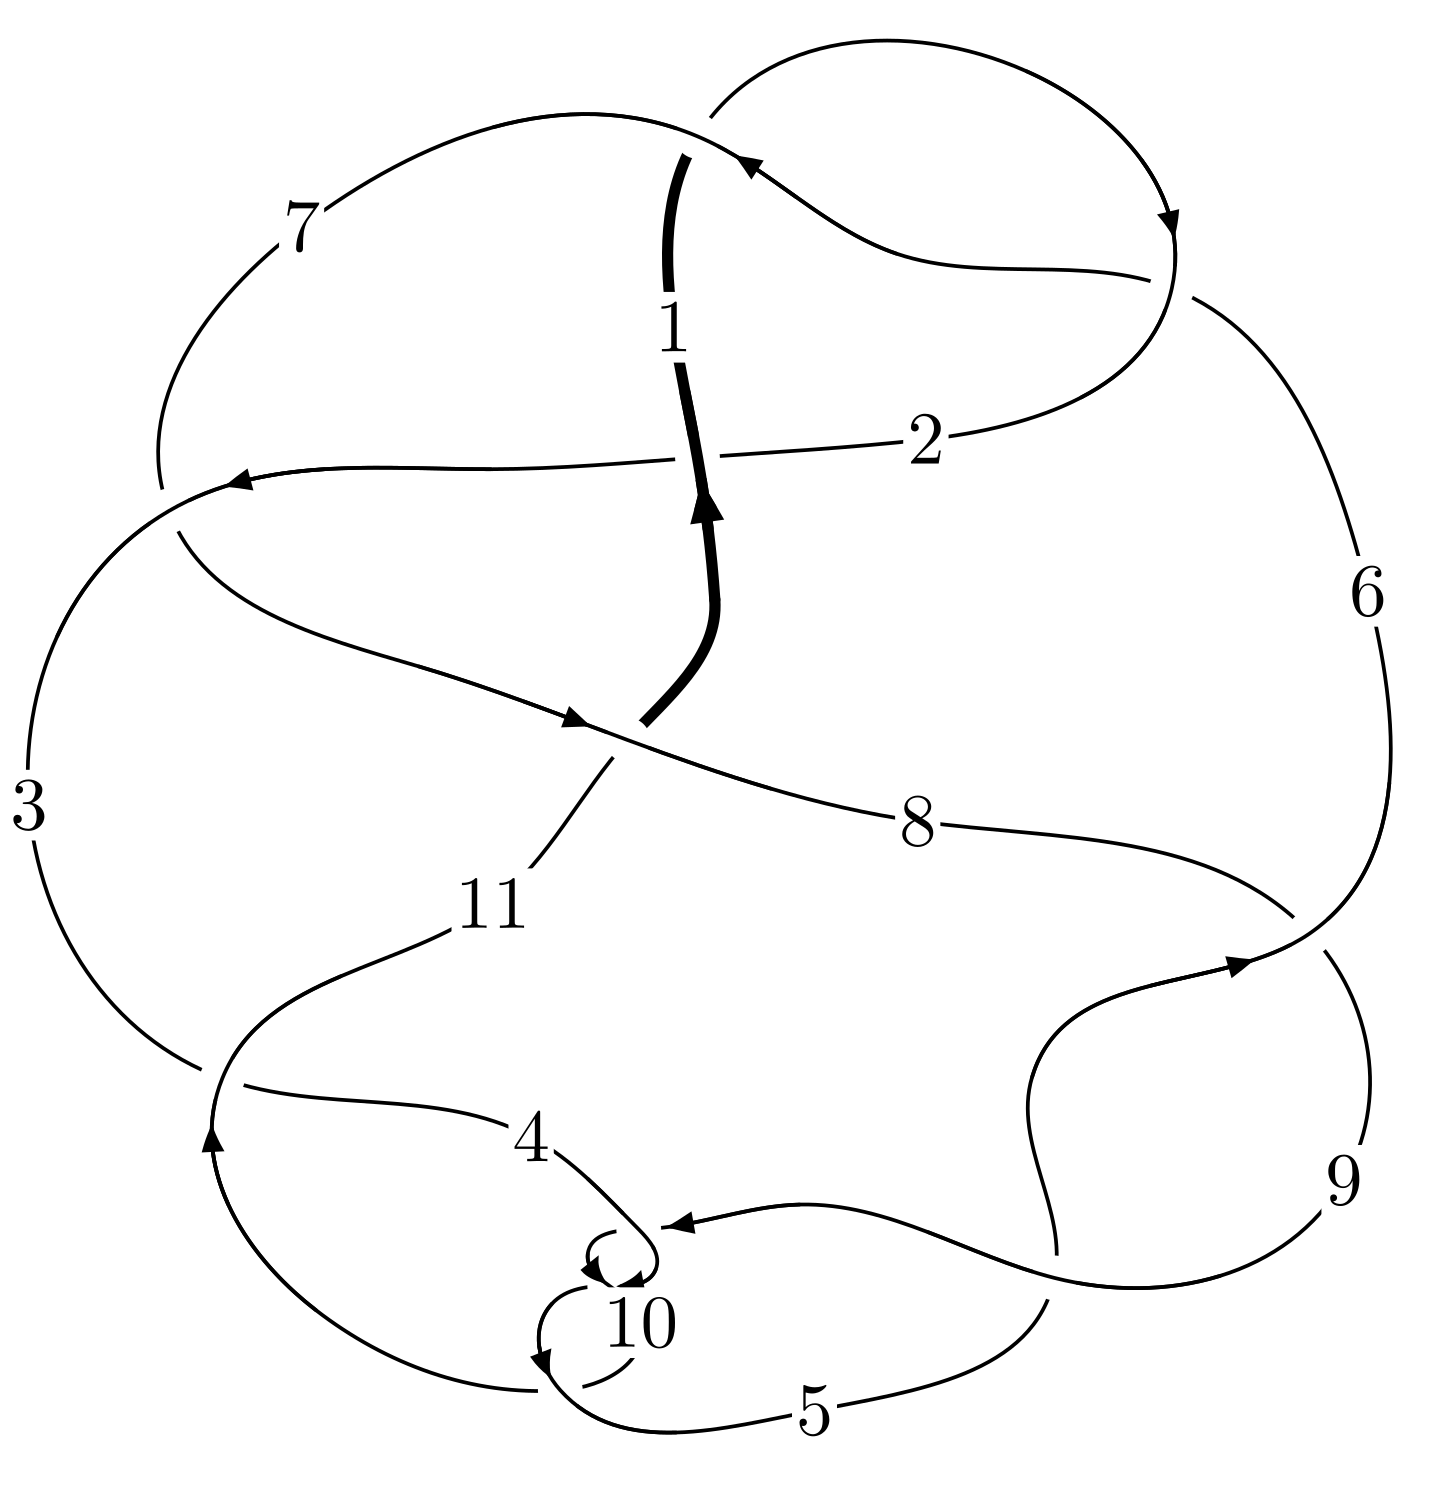
\includegraphics[width=112pt]{../../../GIT/diagram.site/Diagrams/png/442_11a_193.png}\\
\ \ \ A knot diagram\footnotemark}&
\allowdisplaybreaks
\textbf{Linearized knot diagam} \\
\cline{2-2}
 &
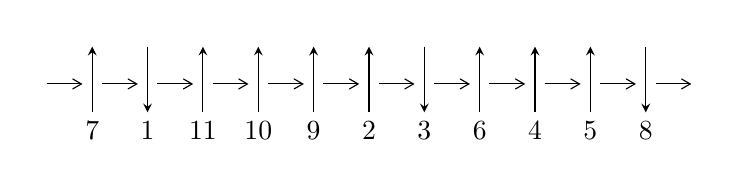
\begin{tikzpicture}[x=20pt, y=17pt]
	% nodes
	\node (C0) at (0, 0) {};
	\node (C1) at (1, 0) {};
	\node (C1U) at (1, +1) {};
	\node (C1D) at (1, -1) {7};

	\node (C2) at (2, 0) {};
	\node (C2U) at (2, +1) {};
	\node (C2D) at (2, -1) {1};

	\node (C3) at (3, 0) {};
	\node (C3U) at (3, +1) {};
	\node (C3D) at (3, -1) {11};

	\node (C4) at (4, 0) {};
	\node (C4U) at (4, +1) {};
	\node (C4D) at (4, -1) {10};

	\node (C5) at (5, 0) {};
	\node (C5U) at (5, +1) {};
	\node (C5D) at (5, -1) {9};

	\node (C6) at (6, 0) {};
	\node (C6U) at (6, +1) {};
	\node (C6D) at (6, -1) {2};

	\node (C7) at (7, 0) {};
	\node (C7U) at (7, +1) {};
	\node (C7D) at (7, -1) {3};

	\node (C8) at (8, 0) {};
	\node (C8U) at (8, +1) {};
	\node (C8D) at (8, -1) {6};

	\node (C9) at (9, 0) {};
	\node (C9U) at (9, +1) {};
	\node (C9D) at (9, -1) {4};

	\node (C10) at (10, 0) {};
	\node (C10U) at (10, +1) {};
	\node (C10D) at (10, -1) {5};

	\node (C11) at (11, 0) {};
	\node (C11U) at (11, +1) {};
	\node (C11D) at (11, -1) {8};
	\node (C12) at (12, 0) {};

	% arrows
	\draw[->,>={angle 60}]
	(C0) edge (C1) (C1) edge (C2) (C2) edge (C3) (C3) edge (C4) (C4) edge (C5) (C5) edge (C6) (C6) edge (C7) (C7) edge (C8) (C8) edge (C9) (C9) edge (C10) (C10) edge (C11) (C11) edge (C12) ;	\draw[->,>=stealth]
	(C1D) edge (C1U) (C2U) edge (C2D) (C3D) edge (C3U) (C4D) edge (C4U) (C5D) edge (C5U) (C6D) edge (C6U) (C7U) edge (C7D) (C8D) edge (C8U) (C9D) edge (C9U) (C10D) edge (C10U) (C11U) edge (C11D) ;
	\end{tikzpicture} \\
\hhline{~~} \\& 
\textbf{Solving Sequence} \\ \cline{2-2} 
 &
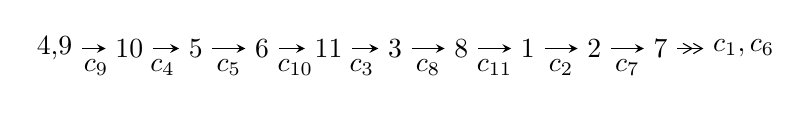
\begin{tikzpicture}[x=24pt, y=7pt]
	% node
	\node (A0) at (-1/8, 0) {4,9};
	\node (A1) at (1, 0) {10};
	\node (A2) at (2, 0) {5};
	\node (A3) at (3, 0) {6};
	\node (A4) at (4, 0) {11};
	\node (A5) at (5, 0) {3};
	\node (A6) at (6, 0) {8};
	\node (A7) at (7, 0) {1};
	\node (A8) at (8, 0) {2};
	\node (A9) at (9, 0) {7};
	\node (C1) at (1/2, -1) {$c_{9}$};
	\node (C2) at (3/2, -1) {$c_{4}$};
	\node (C3) at (5/2, -1) {$c_{5}$};
	\node (C4) at (7/2, -1) {$c_{10}$};
	\node (C5) at (9/2, -1) {$c_{3}$};
	\node (C6) at (11/2, -1) {$c_{8}$};
	\node (C7) at (13/2, -1) {$c_{11}$};
	\node (C8) at (15/2, -1) {$c_{2}$};
	\node (C9) at (17/2, -1) {$c_{7}$};
	\node (A10) at (41/4, 0) {$c_{1},c_{6}$};

	% edge
	\draw[->,>=stealth]	
	(A0) edge (A1) (A1) edge (A2) (A2) edge (A3) (A3) edge (A4) (A4) edge (A5) (A5) edge (A6) (A6) edge (A7) (A7) edge (A8) (A8) edge (A9) ;
	\draw[->>,>={angle 60}]	
	(A9) edge (A10);
\end{tikzpicture} \\ 

\end{tabular} \\

\footnotetext{
The image of knot diagram is generated by the software ``\textbf{Draw programme}" developed by Andrew Bartholomew(\url{http://www.layer8.co.uk/maths/draw/index.htm\#Running-draw}), where we modified some parts for our purpose(\url{https://github.com/CATsTAILs/LinksPainter}).
}\phantom \\ \newline 
\centering \textbf{Ideals for irreducible components\footnotemark of $X_{\text{par}}$} 
 
\begin{align*}
I^u_{1}&=\langle 
u^{47}+u^{46}+\cdots-4 u^3+1\rangle \\
\\
\end{align*}
\raggedright * 1 irreducible components of $\dim_{\mathbb{C}}=0$, with total 47 representations.\\
\footnotetext{All coefficients of polynomials are rational numbers. But the coefficients are sometimes approximated in decimal forms when there is not enough margin.}
\newpage
\renewcommand{\arraystretch}{1}
\centering \section*{I. $I^u_{1}= \langle u^{47}+u^{46}+\cdots-4 u^3+1 \rangle$}
\flushleft \textbf{(i) Arc colorings}\\
\begin{tabular}{m{7pt} m{180pt} m{7pt} m{180pt} }
\flushright $a_{4}=$&$\begin{pmatrix}0\\u\end{pmatrix}$ \\
\flushright $a_{9}=$&$\begin{pmatrix}1\\0\end{pmatrix}$ \\
\flushright $a_{10}=$&$\begin{pmatrix}1\\- u^2\end{pmatrix}$ \\
\flushright $a_{5}=$&$\begin{pmatrix}u\\- u^3+u\end{pmatrix}$ \\
\flushright $a_{6}=$&$\begin{pmatrix}- u^3+2 u\\- u^3+u\end{pmatrix}$ \\
\flushright $a_{11}=$&$\begin{pmatrix}- u^2+1\\u^4-2 u^2\end{pmatrix}$ \\
\flushright $a_{3}=$&$\begin{pmatrix}- u^5+2 u^3- u\\u^7-3 u^5+2 u^3+u\end{pmatrix}$ \\
\flushright $a_{8}=$&$\begin{pmatrix}u^6-3 u^4+2 u^2+1\\u^6-2 u^4+u^2\end{pmatrix}$ \\
\flushright $a_{1}=$&$\begin{pmatrix}- u^{16}+7 u^{14}-19 u^{12}+22 u^{10}-3 u^8-14 u^6+6 u^4+2 u^2+1\\- u^{16}+6 u^{14}-14 u^{12}+14 u^{10}-2 u^8-6 u^6+4 u^4-2 u^2\end{pmatrix}$ \\
\flushright $a_{2}=$&$\begin{pmatrix}u^{39}-16 u^{37}+\cdots+24 u^5+6 u^3\\u^{39}-15 u^{37}+\cdots-3 u^5+u\end{pmatrix}$ \\
\flushright $a_{7}=$&$\begin{pmatrix}u^{18}-7 u^{16}+20 u^{14}-27 u^{12}+11 u^{10}+13 u^8-14 u^6+3 u^2+1\\- u^{20}+8 u^{18}-26 u^{16}+40 u^{14}-19 u^{12}-24 u^{10}+30 u^8-9 u^4\end{pmatrix}$\\ \flushright $a_{7}=$&$\begin{pmatrix}u^{18}-7 u^{16}+20 u^{14}-27 u^{12}+11 u^{10}+13 u^8-14 u^6+3 u^2+1\\- u^{20}+8 u^{18}-26 u^{16}+40 u^{14}-19 u^{12}-24 u^{10}+30 u^8-9 u^4\end{pmatrix}$\\&\end{tabular}
\flushleft \textbf{(ii) Obstruction class $= -1$}\\~\\
\flushleft \textbf{(iii) Cusp Shapes $= -4 u^{44}+68 u^{42}+\cdots-8 u^2+2$}\\~\\
\newpage\renewcommand{\arraystretch}{1}
\flushleft \textbf{(iv) u-Polynomials at the component}\newline \\
\begin{tabular}{m{50pt}|m{274pt}}
Crossings & \hspace{64pt}u-Polynomials at each crossing \\
\hline $$\begin{aligned}c_{1},c_{6}\end{aligned}$$&$\begin{aligned}
&u^{47}+u^{46}+\cdots-2 u^4-1
\end{aligned}$\\
\hline $$\begin{aligned}c_{2}\end{aligned}$$&$\begin{aligned}
&u^{47}+23 u^{46}+\cdots-4 u^2-1
\end{aligned}$\\
\hline $$\begin{aligned}c_{3},c_{5},c_{8}\end{aligned}$$&$\begin{aligned}
&u^{47}+3 u^{46}+\cdots+8 u+1
\end{aligned}$\\
\hline $$\begin{aligned}c_{4},c_{9},c_{10}\end{aligned}$$&$\begin{aligned}
&u^{47}- u^{46}+\cdots-4 u^3-1
\end{aligned}$\\
\hline $$\begin{aligned}c_{7}\end{aligned}$$&$\begin{aligned}
&u^{47}- u^{46}+\cdots-22 u-53
\end{aligned}$\\
\hline $$\begin{aligned}c_{11}\end{aligned}$$&$\begin{aligned}
&u^{47}+5 u^{46}+\cdots-64 u-16
\end{aligned}$\\
\hline
\end{tabular}\\~\\
\newpage\renewcommand{\arraystretch}{1}
\flushleft \textbf{(v) Riley Polynomials at the component}\newline \\
\begin{tabular}{m{50pt}|m{274pt}}
Crossings & \hspace{64pt}Riley Polynomials at each crossing \\
\hline $$\begin{aligned}c_{1},c_{6}\end{aligned}$$&$\begin{aligned}
&y^{47}+23 y^{46}+\cdots-4 y^2-1
\end{aligned}$\\
\hline $$\begin{aligned}c_{2}\end{aligned}$$&$\begin{aligned}
&y^{47}+3 y^{46}+\cdots-8 y-1
\end{aligned}$\\
\hline $$\begin{aligned}c_{3},c_{5},c_{8}\end{aligned}$$&$\begin{aligned}
&y^{47}+47 y^{46}+\cdots-8 y-1
\end{aligned}$\\
\hline $$\begin{aligned}c_{4},c_{9},c_{10}\end{aligned}$$&$\begin{aligned}
&y^{47}-37 y^{46}+\cdots-16 y^2-1
\end{aligned}$\\
\hline $$\begin{aligned}c_{7}\end{aligned}$$&$\begin{aligned}
&y^{47}-17 y^{46}+\cdots+47124 y-2809
\end{aligned}$\\
\hline $$\begin{aligned}c_{11}\end{aligned}$$&$\begin{aligned}
&y^{47}-5 y^{46}+\cdots+1312 y-256
\end{aligned}$\\
\hline
\end{tabular}\\~\\
\newpage\flushleft \textbf{(vi) Complex Volumes and Cusp Shapes}
$$\begin{array}{c|c|c}  
\text{Solutions to }I^u_{1}& \I (\text{vol} + \sqrt{-1}CS) & \text{Cusp shape}\\
 \hline 
\begin{aligned}
u &= \phantom{-}1.006280 + 0.120689 I\end{aligned}
 & -0.91501 + 3.60507 I & \phantom{-}1.64705 - 4.50144 I \\ \hline\begin{aligned}
u &= \phantom{-}1.006280 - 0.120689 I\end{aligned}
 & -0.91501 - 3.60507 I & \phantom{-}1.64705 + 4.50144 I \\ \hline\begin{aligned}
u &= -1.10074\phantom{ +0.000000I}\end{aligned}
 & \phantom{-}1.86864\phantom{ +0.000000I} & \phantom{-}5.66480\phantom{ +0.000000I} \\ \hline\begin{aligned}
u &= \phantom{-}0.030039 + 0.875142 I\end{aligned}
 & -10.56620 + 0.61135 I & -3.63402 + 0.19416 I \\ \hline\begin{aligned}
u &= \phantom{-}0.030039 - 0.875142 I\end{aligned}
 & -10.56620 - 0.61135 I & -3.63402 - 0.19416 I \\ \hline\begin{aligned}
u &= \phantom{-}0.055754 + 0.872511 I\end{aligned}
 & -8.79586 + 8.79339 I & -1.19946 - 6.11283 I \\ \hline\begin{aligned}
u &= \phantom{-}0.055754 - 0.872511 I\end{aligned}
 & -8.79586 - 8.79339 I & -1.19946 + 6.11283 I \\ \hline\begin{aligned}
u &= -0.047289 + 0.862249 I\end{aligned}
 & -6.19361 - 3.85394 I & \phantom{-}1.82254 + 2.54256 I \\ \hline\begin{aligned}
u &= -0.047289 - 0.862249 I\end{aligned}
 & -6.19361 + 3.85394 I & \phantom{-}1.82254 - 2.54256 I \\ \hline\begin{aligned}
u &= -0.021231 + 0.815572 I\end{aligned}
 & -3.88334 - 2.31182 I & \phantom{-}2.62267 + 3.54472 I \\ \hline\begin{aligned}
u &= -0.021231 - 0.815572 I\end{aligned}
 & -3.88334 + 2.31182 I & \phantom{-}2.62267 - 3.54472 I \\ \hline\begin{aligned}
u &= -1.257110 + 0.182931 I\end{aligned}
 & \phantom{-}1.02961 - 1.77431 I & \phantom{-0.000000 } 0 \\ \hline\begin{aligned}
u &= -1.257110 - 0.182931 I\end{aligned}
 & \phantom{-}1.02961 + 1.77431 I & \phantom{-0.000000 } 0 \\ \hline\begin{aligned}
u &= \phantom{-}1.223180 + 0.419244 I\end{aligned}
 & -5.19614 - 4.16894 I & \phantom{-0.000000 } 0 \\ \hline\begin{aligned}
u &= \phantom{-}1.223180 - 0.419244 I\end{aligned}
 & -5.19614 + 4.16894 I & \phantom{-0.000000 } 0 \\ \hline\begin{aligned}
u &= -1.230390 + 0.406583 I\end{aligned}
 & -2.54267 - 0.69419 I & \phantom{-0.000000 } 0 \\ \hline\begin{aligned}
u &= -1.230390 - 0.406583 I\end{aligned}
 & -2.54267 + 0.69419 I & \phantom{-0.000000 } 0 \\ \hline\begin{aligned}
u &= -1.259550 + 0.357794 I\end{aligned}
 & -0.05039 - 1.90652 I & \phantom{-0.000000 } 0 \\ \hline\begin{aligned}
u &= -1.259550 - 0.357794 I\end{aligned}
 & -0.05039 + 1.90652 I & \phantom{-0.000000 } 0 \\ \hline\begin{aligned}
u &= \phantom{-}1.249070 + 0.416752 I\end{aligned}
 & -6.79512 + 4.01291 I & \phantom{-0.000000 } 0 \\ \hline\begin{aligned}
u &= \phantom{-}1.249070 - 0.416752 I\end{aligned}
 & -6.79512 - 4.01291 I & \phantom{-0.000000 } 0 \\ \hline\begin{aligned}
u &= \phantom{-}1.316370 + 0.096272 I\end{aligned}
 & \phantom{-}5.85726 + 2.05767 I & \phantom{-0.000000 } 0 \\ \hline\begin{aligned}
u &= \phantom{-}1.316370 - 0.096272 I\end{aligned}
 & \phantom{-}5.85726 - 2.05767 I & \phantom{-0.000000 } 0 \\ \hline\begin{aligned}
u &= -1.324170 + 0.059973 I\end{aligned}
 & \phantom{-}4.48508 + 2.49902 I & \phantom{-0.000000 } 0 \\ \hline\begin{aligned}
u &= -1.324170 - 0.059973 I\end{aligned}
 & \phantom{-}4.48508 - 2.49902 I & \phantom{-0.000000 } 0 \\ \hline\begin{aligned}
u &= \phantom{-}1.319560 + 0.153160 I\end{aligned}
 & \phantom{-}5.16266 + 3.85903 I & \phantom{-0.000000 } 0 \\ \hline\begin{aligned}
u &= \phantom{-}1.319560 - 0.153160 I\end{aligned}
 & \phantom{-}5.16266 - 3.85903 I & \phantom{-0.000000 } 0 \\ \hline\begin{aligned}
u &= \phantom{-}1.288740 + 0.366736 I\end{aligned}
 & \phantom{-}0.19960 + 6.56847 I & \phantom{-0.000000 } 0 \\ \hline\begin{aligned}
u &= \phantom{-}1.288740 - 0.366736 I\end{aligned}
 & \phantom{-}0.19960 - 6.56847 I & \phantom{-0.000000 } 0 \\ \hline\begin{aligned}
u &= -1.331010 + 0.174169 I\end{aligned}
 & \phantom{-}3.09173 - 8.65002 I & \phantom{-0.000000 } 0\\
 \hline 
 \end{array}$$\newpage$$\begin{array}{c|c|c}  
\text{Solutions to }I^u_{1}& \I (\text{vol} + \sqrt{-1}CS) & \text{Cusp shape}\\
 \hline 
\begin{aligned}
u &= -1.331010 - 0.174169 I\end{aligned}
 & \phantom{-}3.09173 + 8.65002 I & \phantom{-0.000000 } 0 \\ \hline\begin{aligned}
u &= -1.298060 + 0.405269 I\end{aligned}
 & -6.42755 - 5.19896 I & \phantom{-0.000000 } 0 \\ \hline\begin{aligned}
u &= -1.298060 - 0.405269 I\end{aligned}
 & -6.42755 + 5.19896 I & \phantom{-0.000000 } 0 \\ \hline\begin{aligned}
u &= \phantom{-}1.308420 + 0.393753 I\end{aligned}
 & -1.96046 + 8.36038 I & \phantom{-0.000000 } 0 \\ \hline\begin{aligned}
u &= \phantom{-}1.308420 - 0.393753 I\end{aligned}
 & -1.96046 - 8.36038 I & \phantom{-0.000000 } 0 \\ \hline\begin{aligned}
u &= -1.315440 + 0.399117 I\end{aligned}
 & -4.51106 - 13.35320 I & \phantom{-0.000000 } 0 \\ \hline\begin{aligned}
u &= -1.315440 - 0.399117 I\end{aligned}
 & -4.51106 + 13.35320 I & \phantom{-0.000000 } 0 \\ \hline\begin{aligned}
u &= \phantom{-}0.283978 + 0.527411 I\end{aligned}
 & -1.92558 + 6.21305 I & \phantom{-}1.17116 - 8.71697 I \\ \hline\begin{aligned}
u &= \phantom{-}0.283978 - 0.527411 I\end{aligned}
 & -1.92558 - 6.21305 I & \phantom{-}1.17116 + 8.71697 I \\ \hline\begin{aligned}
u &= \phantom{-}0.146756 + 0.548854 I\end{aligned}
 & -3.20832 - 0.82330 I & -2.58409 - 0.88162 I \\ \hline\begin{aligned}
u &= \phantom{-}0.146756 - 0.548854 I\end{aligned}
 & -3.20832 + 0.82330 I & -2.58409 + 0.88162 I \\ \hline\begin{aligned}
u &= \phantom{-}0.519306 + 0.197953 I\end{aligned}
 & -0.86762 - 3.28146 I & \phantom{-}4.49365 + 2.23360 I \\ \hline\begin{aligned}
u &= \phantom{-}0.519306 - 0.197953 I\end{aligned}
 & -0.86762 + 3.28146 I & \phantom{-}4.49365 - 2.23360 I \\ \hline\begin{aligned}
u &= -0.266858 + 0.458418 I\end{aligned}
 & \phantom{-}0.27118 - 1.71840 I & \phantom{-}4.99592 + 5.33344 I \\ \hline\begin{aligned}
u &= -0.266858 - 0.458418 I\end{aligned}
 & \phantom{-}0.27118 + 1.71840 I & \phantom{-}4.99592 - 5.33344 I \\ \hline\begin{aligned}
u &= -0.345961 + 0.277574 I\end{aligned}
 & \phantom{-}0.861649 - 0.739192 I & \phantom{-}8.37308 + 5.15460 I \\ \hline\begin{aligned}
u &= -0.345961 - 0.277574 I\end{aligned}
 & \phantom{-}0.861649 + 0.739192 I & \phantom{-}8.37308 - 5.15460 I\\
 \hline 
 \end{array}$$\newpage
\newpage\renewcommand{\arraystretch}{1}
\centering \section*{ II. u-Polynomials}
\begin{tabular}{m{50pt}|m{274pt}}
Crossings & \hspace{64pt}u-Polynomials at each crossing \\
\hline $$\begin{aligned}c_{1},c_{6}\end{aligned}$$&$\begin{aligned}
&u^{47}+u^{46}+\cdots-2 u^4-1
\end{aligned}$\\
\hline $$\begin{aligned}c_{2}\end{aligned}$$&$\begin{aligned}
&u^{47}+23 u^{46}+\cdots-4 u^2-1
\end{aligned}$\\
\hline $$\begin{aligned}c_{3},c_{5},c_{8}\end{aligned}$$&$\begin{aligned}
&u^{47}+3 u^{46}+\cdots+8 u+1
\end{aligned}$\\
\hline $$\begin{aligned}c_{4},c_{9},c_{10}\end{aligned}$$&$\begin{aligned}
&u^{47}- u^{46}+\cdots-4 u^3-1
\end{aligned}$\\
\hline $$\begin{aligned}c_{7}\end{aligned}$$&$\begin{aligned}
&u^{47}- u^{46}+\cdots-22 u-53
\end{aligned}$\\
\hline $$\begin{aligned}c_{11}\end{aligned}$$&$\begin{aligned}
&u^{47}+5 u^{46}+\cdots-64 u-16
\end{aligned}$\\
\hline
\end{tabular}\newpage\renewcommand{\arraystretch}{1}
\centering \section*{ III. Riley Polynomials}
\begin{tabular}{m{50pt}|m{274pt}}
Crossings & \hspace{64pt}Riley Polynomials at each crossing \\
\hline $$\begin{aligned}c_{1},c_{6}\end{aligned}$$&$\begin{aligned}
&y^{47}+23 y^{46}+\cdots-4 y^2-1
\end{aligned}$\\
\hline $$\begin{aligned}c_{2}\end{aligned}$$&$\begin{aligned}
&y^{47}+3 y^{46}+\cdots-8 y-1
\end{aligned}$\\
\hline $$\begin{aligned}c_{3},c_{5},c_{8}\end{aligned}$$&$\begin{aligned}
&y^{47}+47 y^{46}+\cdots-8 y-1
\end{aligned}$\\
\hline $$\begin{aligned}c_{4},c_{9},c_{10}\end{aligned}$$&$\begin{aligned}
&y^{47}-37 y^{46}+\cdots-16 y^2-1
\end{aligned}$\\
\hline $$\begin{aligned}c_{7}\end{aligned}$$&$\begin{aligned}
&y^{47}-17 y^{46}+\cdots+47124 y-2809
\end{aligned}$\\
\hline $$\begin{aligned}c_{11}\end{aligned}$$&$\begin{aligned}
&y^{47}-5 y^{46}+\cdots+1312 y-256
\end{aligned}$\\
\hline
\end{tabular}
\vskip 2pc
\end{document}